\documentclass[11pt]{article}
%
%--------------------   start of the 'preamble'
%
\usepackage{fullpage}
\usepackage[latin1]{inputenc}
\usepackage[T1]{fontenc}
\usepackage{lmodern}
\usepackage{amsmath}
\usepackage{amsfonts}
\usepackage{amssymb}
\usepackage[bookmarks=true,bookmarksnumbered=true,colorlinks=false,pdfborder={0 0 0}]{hyperref}
\usepackage{picinpar, wrapfig}
\usepackage{array, multirow, hhline, tabularx, graphicx}

\usepackage{cite}

\numberwithin{equation}{section}
\numberwithin{figure}{section}
\numberwithin{table}{section}

\begin{document}

{\bf Report:} Decomposition in different modes. {\bf Authors:} ...

\begin{abstract}

abstract

\section{Introduction}

Numerous traffic estimation techniques developed in the literature rely on density based traffic models such as the Lighthill-Whitham-Richards (LWR) partial differential equation (PDE) \cite{Lighthill1955,Richards1956} and its discretization using the Godunov scheme \cite{Lebacque1996,LeVeque1992,Strub2006} (also known as the Cell Transmission Model (CTM) \cite{Daganzo1994,Daganzo1995} in the transportation literature). These highway traffic monitoring systems rely on large amounts of data from different sources. These include \textit{inductive loop detectors} (ILD) used in the PeMS system \cite{Chen2005} and \textit{in-vehicle transponders} (IVTs) such as FasTrak. Recently, the available data on traffic has increased tremendously since the development of cellular phone based highway traffic monitoring. With the cellular phone communication infrastructure in place and privacy aware smartphone sensing technology in full expansion \cite{Hoh2008}, a large volume of data from mobile devices is now available \cite{Herrera2009}. Large scale Applications include traffic flow estimation to assimilate velocity measurements \cite{Work2008,Work2008a}, which is a rapidly expanding field at the heart of mobile internet services. This points out on the necessity of powerful statistical filters and algorithms to efficiently assimilate the measurements.

In \cite{Work2008,Work2008a}using the \textit{Ensemble Kalman Filter} is used to assimilate velocity measurements. In \cite{Munoz2003}, a switching-mode model (SMM) has been derived from the CTM, which is a nonlinear discrete time dynamical system. This consists in switching among different sets of linear difference equations, defined as linear state-space model (SSM) or modes, combined with a hidden Markov model to describe the transitions from one mode to another. The Mixture Kalman filter algorithm \cite{Chen2000} is employed to assimilate data in a switching state-space model. In this paper, we show that for a Daganzo-Newell fundamental diagram, the Godunov scheme applied to the LWR model (described in \cite{Daganzo1995}) is a piecewise affine (PWA) dynamic system, where each affine component is a linear mode. Contrary to the SMM, where an additional statistical model, namely the hidden Markov model, is introduced, we unravel the PWA character of the original CTM.


\section{Traffic flow modelling}

\subsection{The LWR Model}

Lighthill and Whitham in 1955 \cite{Lighthill1955} introduce a macroscopic dynamic model of traffic based on conservation of cars (\ref{eq:LWRmodel1}), using Greenshields' hypothesis \cite{Greenshields1934} of a static flow/density relationship (\ref{eq:LWRmodel2}), known as the \textit{fundamental diagram}. The model consists of the following two equations:

\begin{equation} \label{eq:LWRmodel1}
\frac{\partial \rho(x,t)}{\partial t} + \frac{\partial q(x,t)}{\partial x} = 0
\end{equation}

\begin{equation} \label{eq:LWRmodel2}
q(x,t) = Q(\rho(x,t))
\end{equation}

\noindent where $\rho(x,t)}$ and $q(x,t)$ denote the density and the flow of vehicles at location x and time t respectively, and $Q$ is the flux function which is assumed to be a function of the density only. 

Equation (\ref{eq:LWRmodel1}) is the principle of conservation of mass, or in this case conservation of vehicles, from fluid dynamics. These equations can be written more compactly as:

\begin{equation} \label{eq:LWRmodel3}
\frac{\partial \rho(x,t)}{\partial t} + Q'(\rho(x,t))\frac{\partial \rho(x,t)}{\partial x} = 0
\end{equation}

This equation is commonly known as the \textit{Lighthill-Whitham-Richards}, or LWR, model. Different fundamental diagrams have been suggested. Greenshields \cite{Greenshields1934} found that freeway speed and density could be reasonably well approximated by a straight line. The expression of the velocity and the flux are then:

\begin{equation} \label{eq:greenshieldsVelocity}
v = V_{G}(\rho) = v_{f}(1-\frac{\rho}{\rho_{j}})
\end{equation}

\begin{equation} \label{eq:greenshieldsFlux}
Q_{G}(\rho) = \rho V_{G}(\rho) = v_{f}(\rho-\frac{\rho^{2}}{\rho_{j}})
\end{equation}

where $v_{f}$ is the free flow (or maximum) velocity, and $\rho_{j}$ is the jam (or maximum) density. In this case, the flow is a quadratic function of the density. 

Many researchers have later suggested alternative shapes that provide a better fit to the measured data. They all share the same characteristics \textbf{LWR1-6}:

LWR1. Greenshields' hypothesis of a static flow/density relationship: $q = Q(\rho(x,t))$

LWR2. $Q(0)=Q(\rho_{j})$=0

LWR3. The continuous portions of $Q(\rho)$ are concave.

LWR4. $V(0) = v_{f}$, and $V(\rho_{j}) = 0$.

LWR5. A critical density $\rho_{c}$ can be defined where the maximum flow $q_{c}$ is attained. Then, $Q(\rho)$ is increasing for $\rho \leq \rho_{c}$ and decrasing for $\rho > \rho_{c}$.

LWR6. The critical density $\rho_{c}$ separates the fundamental diagram into two regimes: \textit{free flow} when $\rho \leq \rho_{c}$ and \textit{congestion} when $\rho > \rho_{c}$

\begin{figure}[here]
  \centering
    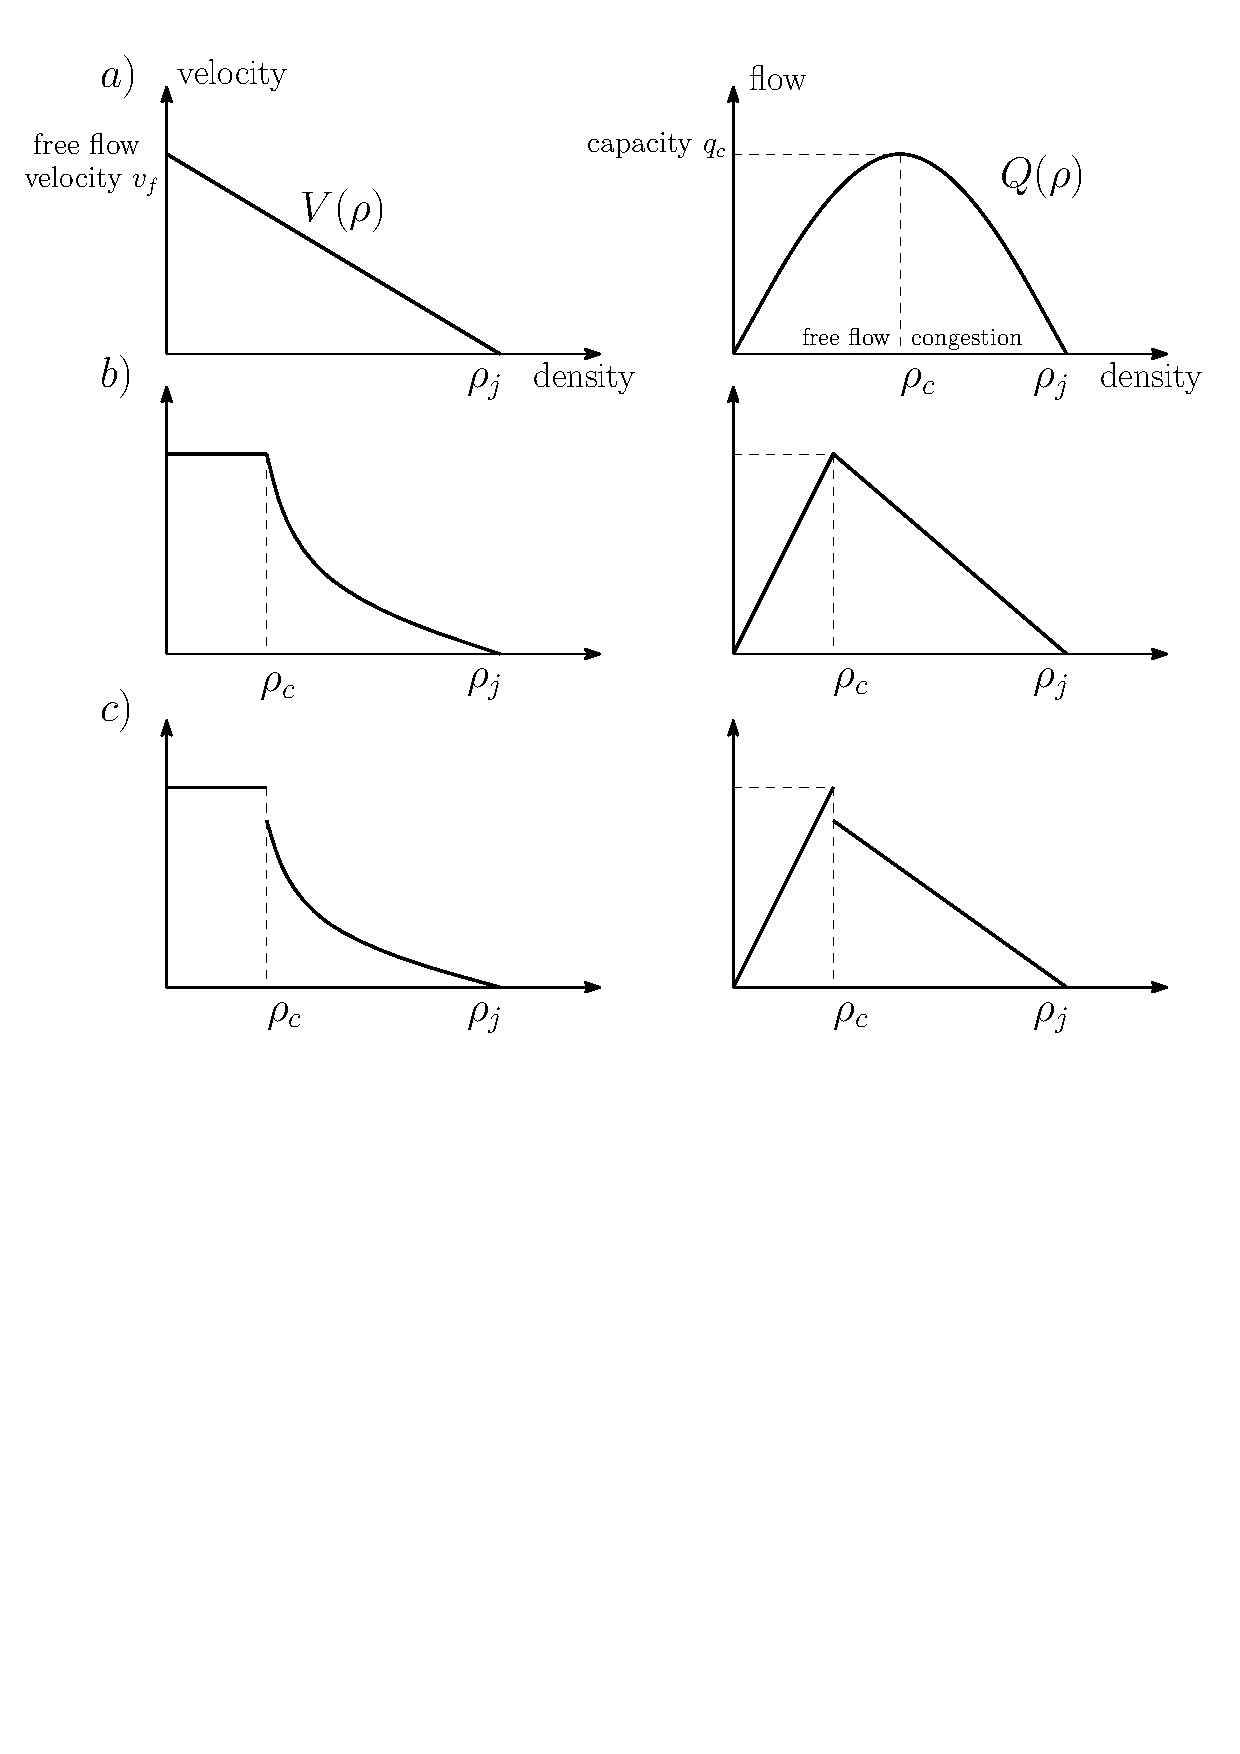
\includegraphics[width=12cm\textwidth]{fundamentalDiagram2.pdf}
    \caption{Speed and flow relationships (fundamental diagrams) for Greenshields (a), Daganzo-Newell (b), and discontinuous (c).}
    \label{fig:fundamentalDiagram}
\end{figure}

Many researchers have later suggested alternative shapes that provide a better fit to the measured data. For instance, the widely used Daganzo-Newell velocity function assumes a constant velocity in free-flow and a hyperbolic velocity in congestion as shown in Figure \ref{fig:fundamentalDiagram}:
\noindent 
\begin{equation}\label{eq:dnVelocity}
v = V_{DN}(\rho) = \left\{ \begin{array}{lcl}
v_{f} & if & \rho \leq \rho_{c} \\
-\omega_{f} \left( 1 - \frac{\rho_{j}}{\rho} \right) & if & \rho > \rho_{c}
\end{array}\right
\end{equation}

\noindent and the corresponding flux function is:

\begin{equation}\label{eq:dnFlux}
Q_{DN}(\rho) = \rho V_{DN}(\rho) \left\{ \begin{array}{lcl}
v_{f} \rho & if & \rho \leq \rho_{c} \\
-\omega_{f} \left( \rho - \rho_{j} \right) & if & \rho > \rho_{c}
\end{array}\right
\end{equation}

\noindent where $\omega_{f}$ is the backwards propagation wave speed.

Measurements on the free-flow side are usually well represented by a straight line, whereas measurements in congestion tend to be more scattered. Some authors claim that there is a difference in the maximum measured flow $Q(\rho_{c})$, depending on whether the freeway is in free-flow or congestion, and contend that a \textit{discontinuity} exists at $\rho=\rho_{c}$ as in Figure \ref{fig:fundamentalDiagram}. This is described in \cite{Agyemang-Duah1991,Cassidy1999,Hall1991} as a \textit{capacity drop}, on the order of 4-10\% in peak flow, as the freeway transitions into congestion.

\subsection{Numerical Discretization}

A good numerical method to solve the equations along roads is represented by the Godunov scheme, which is based on exact solutions to Riemann problems \cite{Godlewski1996,Godunov1959}. This leads to the construction of a nonlinear discrete time dynamical system.

The Godunov discretization scheme is applied on the LWR PDE, where the discrete time step $\Delta T$ is indexed by $t$, and the discrete space step is indexed by $i$:

\begin{equation} \label{eq:rhoGodunov}
\rho^{t+1}_{i} = \rho^{t}_{i} - \frac{\Delta T}{\Delta X}\left(G(\rho^{t}_{i},\rho^{t}_{i+1})-G(\rho^{t}_{i-1},\rho^{t}_{i})\right)
\end{equation}

\noindent In order to ensure numerical stability, the time and space steps are coupled by the CFL condition \cite{LeVeque1992}: $c_{max}\frac{\Delta T}{\Delta X} \leq 1$ where $c_{max}$ denotes the maximal characteristic speed.

For the rest of the paper, the widely-used \textit{Cell Transmission Model} (CTM) described in \cite{Daganzo1994} is chosen for our dynamic model and results are derived from it. For a family of flux functions $Q(\rho)$ that share the same characteristics \textbf{LWR1-6} listed above, the Godunov flux can be expressed as the minimum of the \textit{sending flow} from the upstream cell and the \textit{receiving flow} from the downstream cell through a boundary connecting two cells of a homogeneous road (i.e. the upstream and downstream cells have the same characteristics) \footnotemark. The \textit{sending flow} $S(\rho)$ is equal to the upstream flow if the upstream traffic is in free flow ($\rho \leq \rho_{c}$) or the capacity of the upstream section $q_{c}$ if the upstream traffic is in congestion ($\rho > \rho_{c}$); on the other hand, the \textit{receiving flow} $R(\rho)$ is equal to the capacity of the downstream section if the downstream traffic is in free flow or the downstream flow if the downstream traffic is in congestion. For this model, we note that for an inhomogeneous segment (for instance due to a change in the number of lanes) a fundamental diagram with different parameters is defined at each cell $i$, consequently we add a subscript: $Q_{i}(\rho)$, $S_{i}(\rho)$, $R_{i}(\rho)$ and there is an implicit subscript for $G(\rho_{i},\rho_{i+1})$.

\footnotetext{
There are various definitions of the Godunov flux $G(\rho_{1},\rho_{2})$ in the litterature, notably in \cite{Garavello2006}:

\begin{equation} \label{eq:rhoGodunovFluxGeneral}
G(\rho_{1},\rho_{2}) = \left\{ \begin{array}{lll}
\text{min}_{\rho \in [\rho_{1},\rho_{2}]} Q(\rho) & \text{if} & \rho_{1} \leq \rho_{2}\\
\text{max}_{\rho \in [\rho_{2},\rho_{1}]} Q(\rho) & \text{if} & \rho_{2} \leq \rho_{1}
\end{array}\right
\end{equation}
\noindent This assumes that a fundamental diagram is defined at each boundary between two cells, which differs from the CTM. 
}

\begin{equation} \label{eq:rhoGodunovFlux1}
G(\rho_{1},\rho_{2}) = \text{min}(S_{1}(\rho_{1}),R_{2}(\rho_{2}))
\end{equation}

\begin{equation} \label{eq:sendingFlow1}
S_{1}(\rho) = \left\{ \begin{array}{lll}
Q_{1}(\rho) & \text{if} & \rho \leq \rho_{c1} \\
q_{c1} &  \text{if} & \rho > \rho_{c1}
\end{array}\right
\end{equation}

\begin{equation} \label{eq:receivingFlow1}
R_{2}(\rho) = \left\{ \begin{array}{lll}
q_{c2} & \text{if} & \rho \leq \rho_{c2} \\
Q_{2}(\rho) &  \text{if} & \rho > \rho_{c2}
\end{array}\right
\end{equation}

\noindent where $\rho_{1}$ is the density of the cell upstream and $\rho_{2}$ is the density of the cell downstream. Then sending and receiving flows for the Daganzo-Newell fundamental diagram is:

\begin{equation} \label{eq:sendingFlow2}
S_{1}(\rho) = \left\{ \begin{array}{lll}
v_{f1}\rho & \text{if} & \rho \leq \rho_{c1} \\
q_{c1} &  \text{if} & \rho > \rho_{c1}
\end{array}\right
\end{equation}

\begin{equation} \label{eq:receivingFlow2}
R_{2}(\rho) = \left\{ \begin{array}{lll}
q_{c2} & \text{if} & \rho \leq \rho_{c2} \\
-\omega_{f2} \left( \rho - \rho_{j2} \right) &  \text{if} & \rho > \rho_{c2}
\end{array}\right
\end{equation}

\begin{figure}[here]
  \centering
    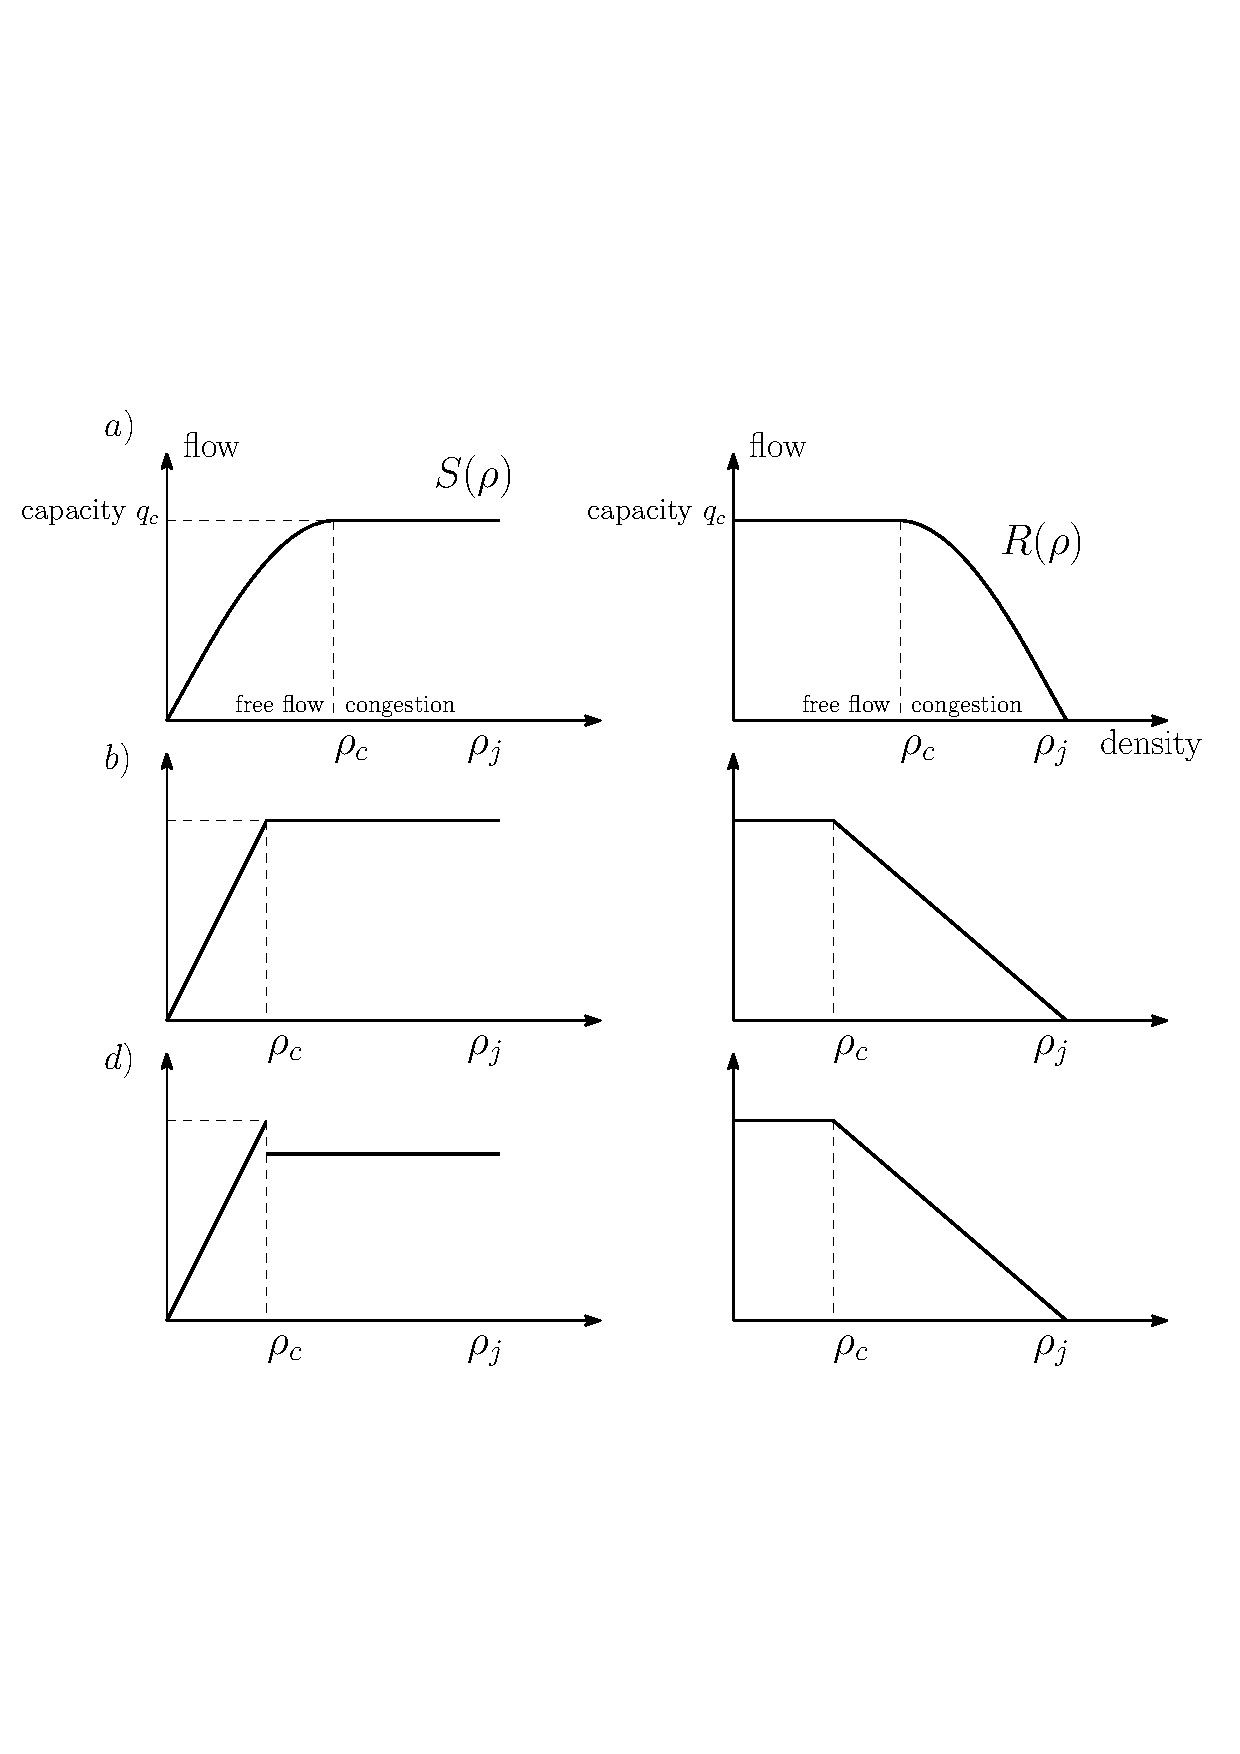
\includegraphics[width=12cm\textwidth]{fundamentalDiagramSR.pdf}
    \caption{Sending and receiving flows for Greenshields (a), Daganzo-Newell (b), and discontinous (c) velocity functions.}
    \label{fig:fundamentalDiagramSR}
\end{figure}

\noindent As shown in Figure \ref{fig:fundamentalDiagramSR}, the application of the Godunov scheme to the fundamental diagrams introduces intuitive concepts of \textit{supply} and \textit{demand} at the boundary connecting two cells. The upstream cell supplies the flow at the boundary up to capicity. We can note that in the discontinuous case, there is a drop in supply capacity when the upstream traffic is in congestion, as described in \cite{Agyemang-Duah1991,Cassidy1999,Hall1991}. As a result, the flow through the boundary is smaller, even if the downstream cell can receive more flow. On the other hand, when the downstream traffic is congested, there is a decrease in demand from the downstream cell, limiting the flow through the boundary. In our paper, we suppose that there is \textit{no capacity drop} through a boundary, i.e. $q_{c1}=q_{c2}=q_{c}$. In Appendix \ref{sec:CDFD}, we discuss the case when $q_{c1}\neq q_{c2}$. In this more general case the results are very similar to the one exposed later.

Figure \ref{fig:godunovDiagram} shows the explicit values taken by $G(\rho_{1},\rho_{2})$ in different regions of the space $(\rho_{1},\rho_{2})$:

\begin{equation}
G(\rho_{1},\rho_{2}) = \left\{ \begin{array}{llll}
R_{2}(\rho_{2}) & \text{if} & (\rho_{1},\rho_{2}) \in \text{white region}\\
q_{c} & \text{if} & (\rho_{1},\rho_{2}) \in \text{light region}\\
S_{1}(\rho_{1}) & \text{if} & (\rho_{1},\rho_{2}) \in \text{dark region}
\end{array}\right
\label{eq:rhoGodunovFlux}
\end{equation}

\begin{equation}
\begin{array}{lll}
\text{white region} & = \{(\rho_{1},\rho_{2}) \mid & \rho_{2} > F(\rho_{1}) \text{ if } \rho_{1} \leq \rho_{c1} \text{, } 
\rho_{2} > \rho_{c2} \text{ if } \rho_{1} > \rho_{c1}\}\\
\text{light region} & = \{(\rho_{1},\rho_{2}) \mid & \rho_{1} > \rho_{c1} \text{ and } \rho_{2} \leq \rho_{c2}\}\\
\text{dark region} & = \{(\rho_{1},\rho_{2}) \mid & \rho_{2} \leq F(\rho_{1}) \text{ and } \rho_{1} \leq \rho_{c1}\}
\end{array}\right
\label{eq:regions}
\end{equation}

\noindent where the boundary between the white and grey regions follows the $(\rho_{1},\rho_{2})=(\rho_{1},F(\rho_{1}))$ trajectory with $F(\rho_{1})= \bar{R}^{-1}_{2}(\bar{S}_{1}(\rho_{1}))$\footnotemark for $\rho_{1} \leq \rho_{c1}$. $\bar{S}$ and $\bar{R}$ denote the restrictions of the sending and receiving flows to the sub-regions $[0,\rho_{c})$ and $(\rho_{c},\rho_{j}]$ respectively, which also correspond to the left and right parts (w.r.t. $\rho_{c}$) of the fundamental diagram, as shown in the Figure \ref{fig:godunovDiagram}.

\footnotetext{Here, we suppose that $\bar{R}$ is a strictly monotonic function on $(\rho_{c},\rho_{j}]$, hence invertible, and $\bar{R}^{-1}$ denotes its inverse.}

\begin{figure}[here]
  \centering
    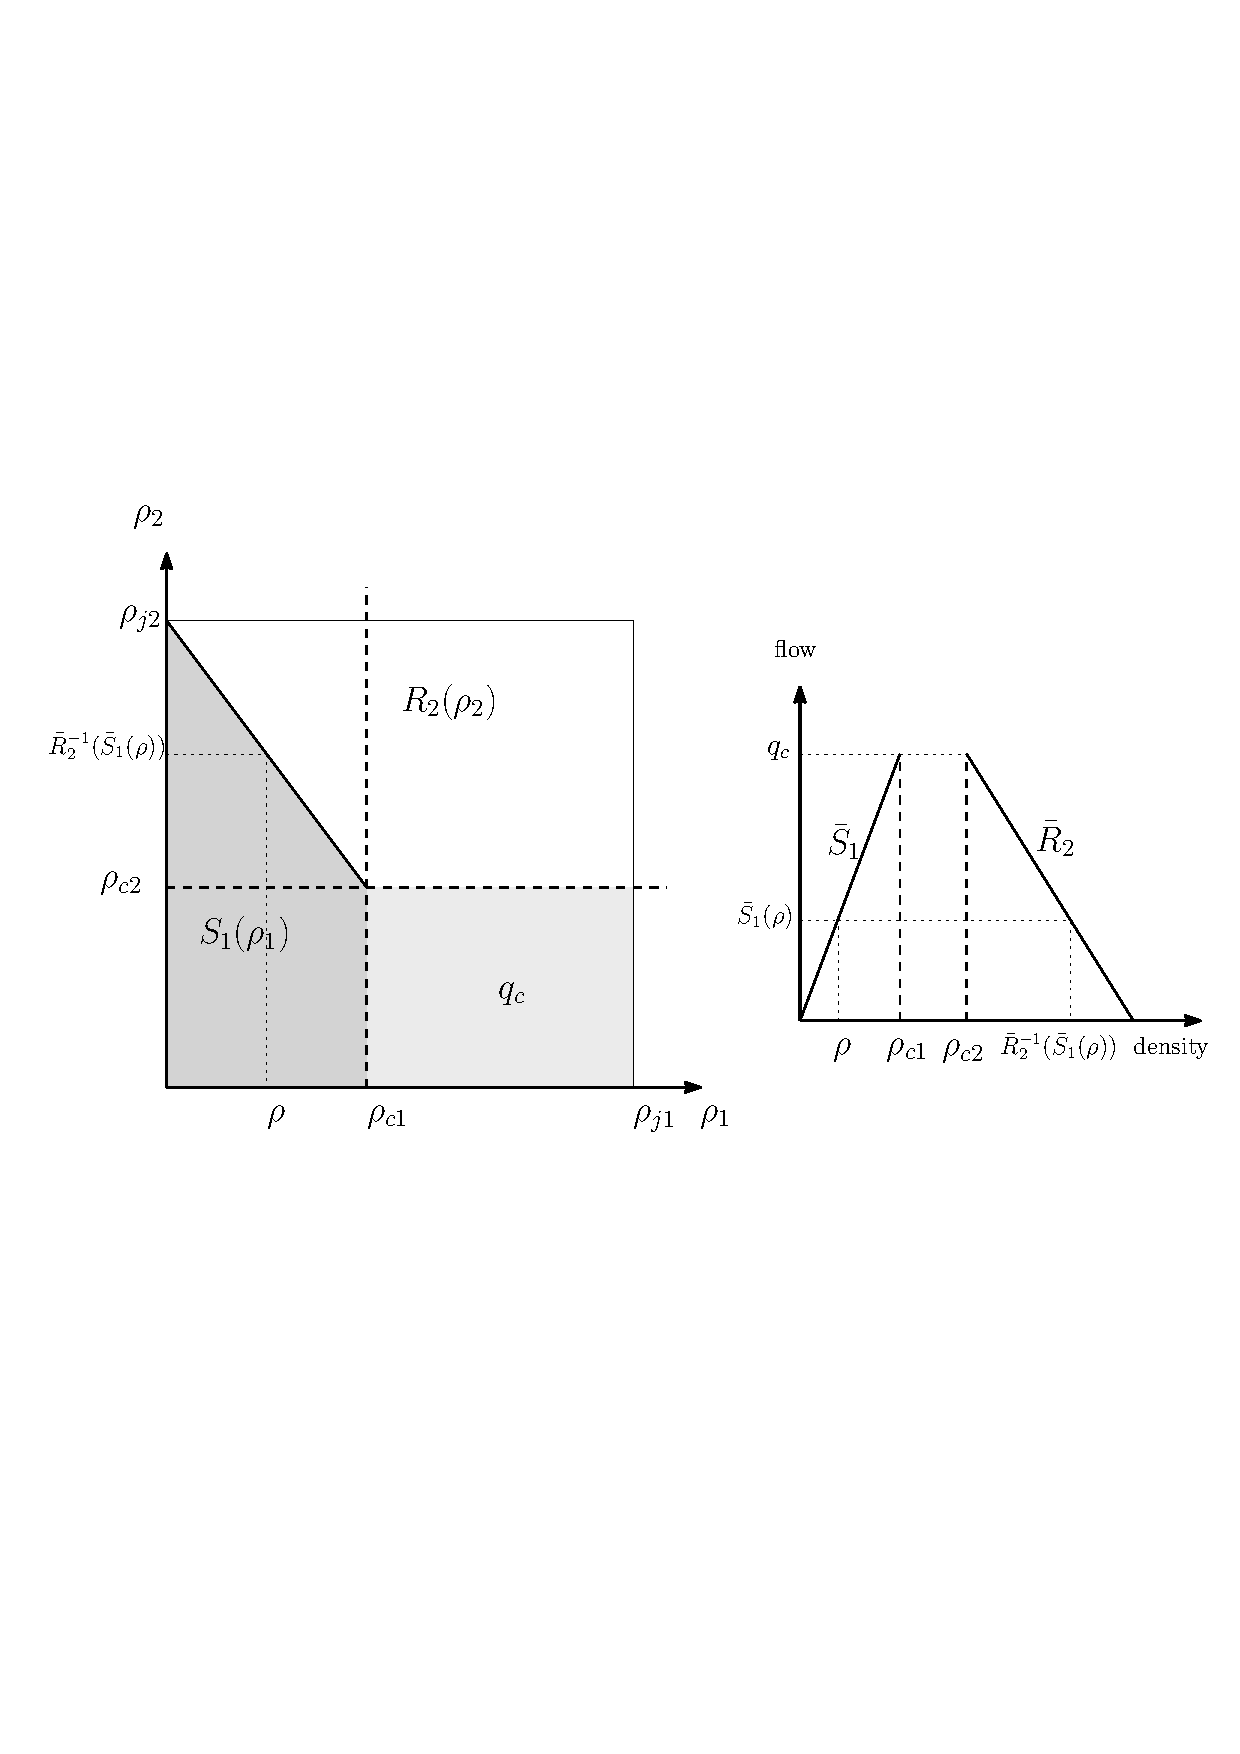
\includegraphics[width=15cm\textwidth]{godunovDiagram2.pdf}
    \caption{Values of $G(\rho_{1},\rho_{2})$ in the space $(\rho_{1},\rho_{2})$ for a family of flux functions with the characteristics \textbf{LWR1-6}, and no capacity drop. Note that for illustration purposes we suppose $\rho_{c1}\leq\rho_{c2}$.}
    \label{fig:godunovDiagram}
\end{figure}

\noindent When the velocity is the Daganzo-Newell function (\ref{eq:dnVelocity}), the Godunov Flux becomes:
\begin{equation} \label{eq:rhoGodunovFlux3}
G_{DN}(\rho_{1},\rho_{2}) = \left\{ \begin{array}{lll}
-\omega_{f2} \left( \rho_{2} - \rho_{j2} \right) & \text{if} & (\rho_{1},\rho_{2}) \in \text{white region}\\
q_{c} & \text{if} & (\rho_{1},\rho_{2}) \in \text{light region}\\
v_{f1} \rho_{1} & \text{if} & (\rho_{1},\rho_{2}) \in \text{dark region}
\end{array}\right
\end{equation}

\noindent and the boundary between the white and grey regions is:

\begin{equation} \label{eq:boundary}
(\rho_{1},\rho_{2})=(\rho_{1},-\frac{v_{f1}}{\omega_{f2}}\rho_{1}+\rho_{j2})
\end{equation}

Subsequently, we will denote by \textbf{W}, \textbf{L}, and \textbf{D} the \textit{white region}, \textit{light region}, and \textit{dark region} of the space $(\rho_{1},\rho_{2})$ respectively. 

\section{Linearization of the Godunov scheme}

In the Godunov scheme (\ref{eq:rhoGodunov}), the update of the density $\rho^{t+1}_{i}$ at $x = i$ depends on the triplet $(\rho^{t}_{i-1}, \rho^{t}_{i}, \rho^{t}_{i+1})$. In this section, we will refer to this triplet as $(\rho_{-}, \rho, \rho_{+})$, $\rho^{t+1}_{i}$ as $\rho^{t+1}$, and the fraction $\frac{\Delta T}{\Delta X}$ as $\alpha$ to ease the notations. Then the Godunov scheme reads as:

\begin{equation} \label{eq:rhoGodunov2}
\rho^{t+1} = f(\rho_{-},\rho,\rho_{+}) = \rho - \alpha\left(G(\rho,\rho_{+})-G(\rho_{-},\rho)\right)
\end{equation}

\subsection{Decomposition in different ''modes''}\label{sec:decompositionModes}

$\rho^{t+1}$ depends on whether both pairs $(\rho_{-}, \rho)$ and $(\rho, \rho_{+})$ are in \textbf{W}, \textbf{L}, or \textbf{D} via $G(\rho_{-},\rho)$ and $G(\rho,\rho_{+})$. So there are nine possible combinations at $x = i$, which can be reduced to seven ''modes'' since the pairs $(\rho_{-}, \rho)$ and $(\rho, \rho_{+})$ have $\rho$ in common. let's denote by $f(\rho_{-},\rho,\rho_{+})$ and $f_{DN}(\rho_{-},\rho,\rho_{+})$ the vector functions for $\rho^{n+1}$ for the general and the Danganzo-Newell cases respectively, which variables are $\rho_{-}$, $\rho$, and $\rho_{+}$. Table \ref{table:modes} list these seven possibilities, which can be easily derived from Figure \ref{fig:godunovDiagram}.

\begin{table}[here]
\centering % used for centering table
\begin{tabular}{c c c c c c} % centered columns (4 columns)
\hline\hline %inserts double horizontal lines
Mode & (\rho_{-}, \rho) & (\rho, \rho_{+}) & $f$(\rho_{-},\rho,\rho_{+}) & $f_{DN}$(\rho_{-},\rho,\rho_{+}) & State \\ [0.5ex]% inserts table
%heading
\hline % inserts single horizontal line
1 & W & W & \rho - \alpha(R_{+}(\rho_{+})-R(\rho)) & (1 - \alpha \omega_{f})\rho + \alpha \omega_{f} \rho_{+} & congestion\\ [1ex]
2 & W & L & \rho - \alpha(q_{c}-R(\rho)) & (1 - \alpha \omega_{f})\rho + \alpha \omega_{f} \rho_{c} & congestion\\ [1ex]
3 & L & W & \rho - \alpha(R_{+}(\rho_{+})-q_{c}) & \rho + \alpha \omega_{f}\rho_{+} - \alpha \omega_{f}\rho_{c} & congestion\\ [1ex]
4 & L & D & \rho - \alpha(S(\rho)-q_{c}) & (1 - \alpha v_{f})\rho + \alpha v_{f} \rho_{c} & free flow\\ [1ex]
5 & D & W & \rho - \alpha(R_{+}(\rho_{+})-S_{-}(\rho_{-})) & \alpha v_{f} \rho_{-} + \rho + \alpha \omega_{f} \rho_{+} - \alpha \omega_{f} \rho_{j} & critical\\ [1ex]
6 & D & L & \rho - \alpha(q_{c}-S_{-}(\rho_{-})) & \alpha v_{f} \rho_{-} + \rho - \alpha v_{f} \rho_{c} & free flow\\ [1ex]
7 & D & D & \rho - \alpha(S(\rho)-S_{-}(\rho_{-})) & \alpha v_{f} \rho_{-} + (1 - \alpha v_{f})\rho & free flow\\ [1ex]% [1ex] adds vertical space
\hline %inserts single line
\end{tabular}
\label{table:modes} % is used to refer this table in the text
\caption{Different values of $\rho^{t+1} = f(\rho_{-},\rho,\rho_{+})$ depending on the values of $G(\rho_{-},\rho)$ and $G(\rho,\rho_{+})$ in the space $(\rho_{1},\rho_{2})$.}
\end{table}

For instance, for the first mode, $(\rho_{-}, \rho)$ and $(\rho, \rho_{+})$ are both in \textbf{W} (cf. Figure \ref{fig:godunovDiagram}), thus $G(\rho_{-}, \rho) = R(\rho)$ and $G(\rho, \rho_{+}) = R_{+}(\rho_{+})$, and then $\rho^{t+1} = f_{1}(\rho_{-},\rho,\rho_{+}) = \rho - \alpha(R_{+}(\rho_{+})-R(\rho))$, where $f_{1}$ is the first entry of $f$. By extending this result to an entire link with discrete state space indexed by $i = 1,...,n$, where $n$ is the number of space steps, we have a whole description of the space of ''modes'' along the link. Since there is a correlation between two consecutive indexes $i$ and $i+1$, the number of modes for the entire link reduces from $3^{n}$ to an expression in the form of $a.\beta^{n} + b.\gamma^{n} + c.\delta^{n}$ which lower and upper bounds are proved to be $3.2^{n}$ and $3.(2.5)^{n}$ respectively (for full details, see Appendix \ref{sec:modes}). Let's denote by $\mathcal{M}_{n}$ the space of modes ($\mathcal{M}_{n}$ \subset $\{1,...,7\}^{n}$). For $m \in \mathcal{M}_{n}$, $m$ is a vector of dimension $n$ which $i-th$ entry $m_{i}\in\{1,...,7\}$ is the mode at cell $i$.

We suppose $\alpha$, $\omega_{f}$, $v_{f}$, $\rho_{j}$, $\rho_{c}$, $q_{c}$ constant w.r.t the time because they are only related to the geometry of the highway, independently of the current traffic on it\footnotemark. We define $J$, the Jacobian matrix of $f$ with respect to $(\rho_{-},\rho,\rho_{+})$:

\footnotetext{
In fact, $\alpha$, $\omega_{f}$, $v_{f}$, $\rho_{j}$, $\rho_{c}$, $q_{c}$ can vary along the link and a proper notation would be $\alpha_{i}$, $\omega_{fi}$, $v_{fi}$, $\rho_{ji}$, $\rho_{ci}$, $q_{ci}$ for the parameters of the fundamental diagram at $x=i$. We choose not to add the subscripts $i$ to simplify the notations.
}

\begin{equation}\label{eq:jacobian}
J = \left(\frac{\partial f_{i}}{\partial \rho_{j}}\right)_{i,j}
\label{eq:jacobian}
\end{equation}

\where $f_{i}$ is the ith entry of the vector function $f$ defined in Table \ref{table:modes}.

It is useful to explicit the Jacobian matrix $J_{DN}$ of the vector function $f_{DN}$ with respect to $(\rho_{-},\rho,\rho_{+})$:

\begin{equation} \label{eq:jacobianDN}
J_{DN} = \begin{pmatrix}
0 & 1 - \alpha \omega_{f} & \alpha \omega_{f+} \\
0 & 1 - \alpha \omega_{f} & 0 \\
0 & 1 & \alpha \omega_{f+} \\
0 &  1 - \alpha v_{f} & 0 \\
\alpha v_{f-} & 1 & \alpha \omega_{f+} \\
\alpha v_{f-} & 1 & 0 \\
\alpha v_{f-} & 1 - \alpha v_{f} & 0
\end{pmatrix} \right
\end{equation}

Since $f_{DN}$ is a \textit{linear function} of $(\rho_{-},\rho,\rho_{+})$ as shown in Table \ref{table:modes}, we can notice that $J_{DN}$ is constant. More notably, we will see in the next section that the decomposition in ''modes'' as shown in Table \ref{table:modes} leads to a linear formulation of the Godunov Scheme in the case of the Daganzo-Newell fundamental diagram, which fits into the Kalman filter framework as we will see in the next section. 

\subsection{Kalman filtering}

Let's consider a link with discrete time step indexed by $t\geq 0$ and discrete space step indexed by $i = 1,...,n$, and let's denote $\boldsymbol\rho^{t} = (\rho^{t}_{0},\rho^{t}_{1},...,\rho^{t}_{n},\rho^{t}_{n+1})$ a n+2 dimensional vector which describes the state of the link at time $t$. $\rho^{t}_{i}$ is the density at time $t$ and cell $i$. We can note that the ghost cells $0$ and $n+1$ are included in the state of the link. $\boldsymbol m^{t}\in\mathcal{M}_{n}$ is the mode of the link at time $t$, as defined in the previous section. At each time increment, the ''true'' state of the link is updated through:

\begin{equation}
\boldsymbol\rho^{t} = F[\boldsymbol\rho^{t-1}]
\label{eq:underlyingSystem1}
\end{equation}

\noindent with $F[.]$ a n+2 dimensional function vector such that the ith entry $F_{i}[\boldsymbol\rho^{t-1}]$ is:

\begin{equation}
\left F_{i}[\boldsymbol\rho^{t-1}] = \left\{ \begin{array}{ll}
f_{m_{i}}(\rho^{t-1}_{i_{-},i,i_{+}}) & \text{for}\quad i=1,...,n\\
\rho^{t}_{0} & \text{for}\quad i=0\\
\rho^{t}_{n+1} & \text{for}\quad i=n+1
\end{array} \right
\label{eq:underlyingSystem2}
\end{equation}

\noindent where $m_{i}$ denotes the ith entry of $\boldsymbol m^{t} \in\mathcal{M}_{n}$ (we omit the subscript $i$ to ease the notations), $f_{m_{i}}(\rho^{t-1}_{i_{-},i,i_{+}})$ is the $m_{i}$-th entry of the function vector $f$ evaluated in $(\rho^{t-1}_{i-1},\rho^{t-1}_{i},\rho^{t-1}_{i+1})$, and $\rho^{t}_{0}$ and $\rho^{t}_{n+1}$ are the boundary conditions upstream and downstream. For a Daganzo-Newell fundamental diagram and a linear-hyperbolic velocity function, the update operators of the dynamic system, namely $F_{DN}[.]$ and $F_{LH}[.]$, have the same expression with $f_{DN}(.)$ and $f_{LH}(.)$ respectively (as defined in Table \ref{table:modesDNandLH}). For instance, when we have a Daganzo-Newell fundamental diagram with update operator for the dynamic system $F_{DN}[.]$ (i.e. $\boldsymbol\rho^{t} = F_{DN}[\boldsymbol\rho^{t-1}]$), and suppose that the mode at $x=i$ is three ($m_{i}=3$) then\footnotemark: 

\begin{equation}
F_{i}[\boldsymbol\rho^{t-1}] = f_{DN,m_{i}}(\rho^{t-1}_{i_{-},i,i_{+}}) = f_{DN,3}(\rho^{t-1}_{i_{-},i,i_{+}}) = 
\rho^{t-1}_{i} + \alpha \omega_{f}\rho^{t-1}_{i+1} - \alpha \omega_{f}\rho_{c}
\label{eq:example}
\end{equation}

\footnotetext{
As we have seen earlier, $\alpha$, $\omega_{f}$, $v_{f}$, $\rho_{j}$, $\rho_{c}$, $q_{c}$ can vary along the link and a proper notation would be $\alpha_{i}$, $\omega_{fi}$, $v_{fi}$, $\rho_{ji}$, $\rho_{ci}$, $q_{ci}$ for the parameters of the fundamental diagram at $x=i$, so that:
\[
F_{i}[\rho^{t-1}] = f_{DN,m_{i}}(\rho^{t-1}_{i_{-},i,i_{+}}) = f_{DN,3}(\rho^{t-1}_{i_{-},i,i_{+}}) = 
\rho^{t-1}_{i} + \alpha_{i} \omega_{fi}\rho^{t-1}_{i+1} - \alpha_{i} \omega_{fi}\rho_{ci}
\]
}

In order to use the \textit{Extended Kalman filter} to estimate the state of the link given a sequence of noisy observations, we model the process in accordance with the framework of the \textit{Extended Kalman filter} by adding a white noise to the underlying dynamic system model. The ''true'' state $\boldsymbol\rho^{t}$ is then:

\begin{equation}
\boldsymbol\rho^{t} = F[\boldsymbol\rho^{t-1}] + \boldsymbol\eta^{t}
\label{eq:underlyingSystem3}
\end{equation}

\noindent where $\boldsymbol\eta^{t}\sim N(0,Q_{t})$ is the Gaussian zero-mean, white state noise with covariance $Q_{t}$. The estimated state at time $t$ is denoted by $\hat{\boldsymbol\rho}^{t}$ and the estimated covariance by $P_{t}$. The \textit{prediction step} gives the \textit{a priori} state estimate and covariance $\hat{\boldsymbol\rho}^{t:t-1}$ and $P_{t:t-1}$:

\begin{equation}
\begin{array}{ll}
\text{Predicted state estimate: } & \hat{\boldsymbol\rho}^{t:t-1} = F[\hat{\boldsymbol\rho}^{t-1}]\\
\text{Predicted covariance estimate: } & P_{t:t-1} = F_{t-1}P_{t-1}(F_{t-1})^{T} + Q_{t-1}
\end{array} \right
\label{eq:predict}
\end{equation}

\noindent where $F_{t}$ is the state transition defined to be the following Jacobian:

\begin{equation}
F_{t} = \left(\frac{\partial \left F_{i}[\rho^{t}]}{\partial \rho^{t}_{j}}\right)_{i,j}
\label{eq:jacobian}
\end{equation}

The estimated mode $\hat{\boldsymbol m}^{t}$ associated to the estimated vector state $\hat{\rho}^{t}$ is defined from Table \ref{table:modes}. Specifically, in the context of our traffic model, the density at $x=i$ only depends on the densities at the neighbor points $x=i-1,i,i+1$. So $F_{t}$ is a $(n+2)\times(n+2)$ tridiagonal matrix, such that the diagonal elements are $\{0, J_{\hat{m}_{1},2},...,J_{\hat{m}_{n},2},0\}$, the lower diagonal elements are $\{J_{\hat{m}_{1},1},J_{\hat{m}_{2},1},...,J_{\hat{m}_{n},1},0\}$, and the upper diagonal elements are $\{0,J_{\hat{m}_{1},3},J_{\hat{m}_{2},3},...,J_{\hat{m}_{n},3}\}$, where $J$ is defined in Equation \ref{eq:jacobian}. 

In the case of the Daganzo-Newell fundamental diagram, the operator $F_{DN}[.]$ defined in (\ref{eq:underlyingSystem2}) is \textit{linear} (from the linearity of $f_{DN}$). Along with the assumption of a white state noise, the \textit{prediction step} (\ref{eq:predict}) of the \textit{Extended Kalman filter} is actually identical to the regular \textit{Kalman filter}, and it is known from the theory that the \textit{Kalman filter} is optimal \cite{Anderson2005}.

In the case of a linear-hyperbolic velocity function, the operator $F_{LH}[.]$ is not linear if at some points of the discrete space the mode is between four and seven. Then the \textit{Extended Kalman filter} is \textit{near-optimal}.

We can note that the first line and first column of $P_{t}$ have only zero elements because the boundary condition $\rho^{t}_{0}$ is deterministic (i.e. $cov(\rho^{t}_{0},\rho^{t}_{i})=0$ for $i=1,...,n$), and similarly the last line and last column of $P_{t}$ are null since the boundary condition $\rho^{t}_{n+1}$ is deteministic. Additionally, the observation model for the link is given by:

\begin{equation}
\boldsymbol y^{t} = H_{t}\boldsymbol\rho^{t} + \boldsymbol\chi^{t}
\label{eq:observation}
\end{equation}

\noindent where $H_{t}\in \{ 0,1 \}^{p_{t}\times n}$ is the linear observation observation matrix which encodes the $p_{t}$ observations (each one of them being at a discrete cell on the highway) for which the density is observed during discrete time step $t$, and $n$ is the number of cells along the link. The last term in (\ref{eq:observation}) is the white, zero mean observation noise $\boldsymbol\chi^{t} \sim N(0,R_{t})$ with covariance matrix $R_{t}$. The \textit{update step} is:

\begin{equation}
\begin{array}{ll}
\text{Kalman gain: } & K_{t} = P_{t:t-1}H_{t}^{T}\left(H_{t}P_{t:t-1}H_{t}^{T}+R_{t}\right)^{-1}\\
\text{Updated state estimate: } & \hat{\boldsymbol\rho}^{t} = \hat{\boldsymbol\rho}^{t:t-1} + K_{t}(\boldsymbol y^{t} - H_{t}\hat{\boldsymbol\rho}^{t:t-1})\\
\text{Updated estimate covariance: } & P_{t} = (I - K_{t}H_{t})P_{t:t-1}
\end{array} \right
\label{eq:predict}
\end{equation}

The Extended Kalman filter provides the distribution of $\hat{\boldsymbol\rho}^{t}$ given the sequence of observations $\boldsymbol y^{0:t}$, sequence of modes $\hat{\boldsymbol m}^{0:t} = \{\hat{\boldsymbol m}^{0},...,\hat{\boldsymbol m}^{t}\}$, and sequence of control parameters $\boldsymbol u^{0:t}$, which is exactly equal to the distribution of $\hat{\boldsymbol\rho}^{t}$ since the sequence $\hat{\boldsymbol m}^{0:t}$ is deterministic. Concretely, the vector of control parameters $\boldsymbol u^{t}$ contain the vector of critical densities $\boldsymbol\rho_{c}$, the vector of jam densities $\boldsymbol\rho_{j}$, and the boundary conditions $\rho^{t}_{0}$ and $\rho^{t}_{n+1}$. Theoretically, the result is obtained by marginalizing the joint distribution of $\hat{\boldsymbol\rho}^{t}$ and $\hat{\boldsymbol m}^{0:t}$ as follows:

\begin{equation}
\begin{array}{ll}
p(\hat{\boldsymbol\rho}^{t}|\boldsymbol y^{0:t},\boldsymbol u_{0:t}) & =
\int_{\mathcal{M}_{n}} p(\hat{\boldsymbol\rho}^{t}|\boldsymbol y^{0:t},\boldsymbol u^{0:t},\boldsymbol m^{0:t})p(\boldsymbol m^{0:t}|\boldsymbol y^{0:t},\boldsymbol u^{0:t})
d\boldsymbol m^{0:t}\\ 
& = \int_{\mathcal{M}_{n}} p(\hat{\boldsymbol\rho}^{t}|\boldsymbol y^{0:t},\boldsymbol u^{0:t},\boldsymbol m^{0:t})\boldsymbol 1_{\hat{\boldsymbol m}^{0:t}}d\boldsymbol m^{0:t}\\[1ex]
& = p(\hat{\boldsymbol\rho}^{t}|\boldsymbol y^{0:t},\boldsymbol u^{0:t},\hat{\boldsymbol m}^{0:t})
\label{eq:marginalization}
\end{array}
\end{equation}

\section{Implementation}

\subsection{Algorithm for the \textit{prediction step}}

Algorithm using the structure of $F_{t}$ and extension to a network

From Appendix \ref{sec:modes},  In (\ref{eq:predict}), the \textit{a priori} state estimate $\hat{\boldsymbol\rho}^{t:t-1}$ is derived through the algorithm in (\ref{eq:underlyingSystem2}).

\subsection{Accuracy}

For a Daganzo-Newell fundamental diagram, we can note that the decomposition in different modes in (\ref{eq:underlyingSystem2}) is in fact a special case of \textit{Conditional Dynamic Linear Model} (CDLM) as described in \cite{Chen2000} with a discrete latent indicator that is deterministic. In this case, there is only one estimated deterministic sequence of modes $\hat{\boldsymbol m}^{0:t}$ or latent indicators, hence there is no need to use a sequential Monte-Carlo method to sample an ensemble of trajectories of modes. The Mixture Kalman Filter \cite{Chen2000} reduces to a simple Kalman Filter. For non-triangular fundamental diagrams which have the characteristics \textbf{LWR1-6}, a first order Taylor Series expansion is applied. Such a linearization is a good approximation, as shown in the example in Appendix \ref{sec:LHFD}. Then the Extended Kalman filter can be applied to each mode.

In our case, the estimated sequence of modes $\hat{\boldsymbol m}^{0:t}$ is readily infered through the Godunov scheme, and at all the cells along the link, including those where there is no observation. Contrary to some previous models as in \cite{Munoz2003}, the modes are not directly sampled from density measurements along the highway. However, the mode is still indirectly infered from those measurements by assimilating the observations with the \textit{update state} of the Kalman filter. Besides, we rely on the accuracy of the estimation of the mode provided by the Godunov scheme when we apply the Kalman filter for each mode. Such an assumption that favors the mode provided by the Godunov scheme is yet another reason why the sequential Monte-Carlo method (with the resampling step) is not used in the algorithm, because we then suppose that our sequence of modes is the one with the largest likelihoods. (to develop, do a test of likelihood)

\subsection{Complexity}

Comparison with the Extended Kalman filter and matlab simulations and results

\section{Conclusion and Future Work}



\section{Acknowledgement}

\appendix

\section{Description of the state of modes}\label{sec:modes}

For an entire link with discrete state space indexed by $i = 1,...,n$ we have a whole description of the space of ''modes'' along it. Since there is always the entry $\rho_{i}$ in common for successive pairs $(\rho_{i-1},\rho_{i})$ and $(\rho_{i},\rho_{i+1})$, a correlation propagates along the link, reducing the number of modes to a quantity smaller than $3^{n}$. 

More precisely, suppose that the pair $(\rho_{0},\rho_{1})$ is in the region \textbf{W}, then the list of possible combinations in Table \ref{table:modes} shows that $(\rho_{1},\rho_{2})$ can be either in \textbf{W} or \textbf{L}. Similarly, if $(\rho_{0},\rho_{1})$ is in the region \textbf{L}, $(\rho_{1},\rho_{2})$ can be either in \textbf{W} or \textbf{L}, and for $(\rho_{0},\rho_{1})$ in \textbf{D}, $(\rho_{1},\rho_{2})$ can be either in \textbf{W}, \textbf{L}, or \textbf{D}. As an example, Table \ref{table:threeLevelModes} describes all the possible sixteen combinations for the first three pairs $(\rho_{0},\rho_{1})$, $(\rho_{1},\rho_{2})$, and $(\rho_{2},\rho_{3})$.

\begin{table}[here]
\centering % used for centering table
\begin{tabular}{|c|c|c|c|c|c|c|c|c|c|c|c|c|c|c|c|c|}
  \hline
  (\rho_{0},\rho_{1}) & \multicolumn{4}{|c|}{W} & \multicolumn{5}{|c|}{L} & \multicolumn{7}{|c|}{D}\\
  \hline
  (\rho_{1},\rho_{2}) & \multicolumn{2}{|c|}{W} & \multicolumn{2}{|c|}{L} & \multicolumn{2}{|c|}{W} & \multicolumn{3}{|c|}{D} & \multicolumn{2}{|c|}{W} & \multicolumn{2}{|c|}{L} & \multicolumn{3}{|c|}{D}\\
  \hline
  (\rho_{2},\rho_{3}) & W & L & W & D & W & L & W & L & D & W & L & W & D & W & L & D\\
  \hline
\end{tabular}
\label{table:threeLevelModes} % is used to refer this table in the text
\caption{Different values of $\rho^{n+1}$ depending on the values of $G(\rho_{-},\rho)$ and $G(\rho,\rho_{+})$ in the space $(\rho_{1},\rho_{2})$ for the Daganzo-Newell fundamental diagram and the Linear-hyperbolic velocity function.}
\end{table}

We can recursively compute the number of ''modes'' $M_{n}$ with respect to $n$, where $n$ is the number of cells of the discretized link. Let's denote by $w_{n}$, $l_{n}$, and $d_{n}$ the number of modes for which $(\rho_{k},\rho_{k+1})$ is in \textbf{W}, \textbf{L}, and \textbf{D} respectively. Then we have these equations: 

\begin{equation}
w_{0} = l_{0} = d_{0} = 1
\label{eq:modes1}
\end{equation}

\begin{equation}
\begin{array}{lllllll}
w_{k+1} & = & w_{k} & + & l_{k} & + & d_{k}\\
l_{k+1} & = & w_{k} & + & d_{k} & & \\
d_{k+1} & = & l_{k} & + & d_{k} & &
\end{array}\right \quad \text{for }k \geq 0
\label{eq:modes2}
\end{equation}

\begin{equation}
n_{k} = w_{k} + l_{k} + d_{k} \quad \text{for }k \geq 0
\label{eq:modes3}
\end{equation}

Using matrix notations, equation (\ref{eq:modes2}) reads:

\begin{equation}
\left[ \begin{array}{c}
w_{k+1} \\
l_{k+1} \\
d_{k+1} \end{array} \right] = A \times 
\left[ \begin{array}{c}
w_{k} \\
l_{k} \\
d_{k} \end{array} \right]
\quad\text{where}\quad A = \left[ \begin{array}{ccc}
1 & 1 & 1 \\
1 & 0 & 1 \\
0 & 1 & 1 \end{array} \right]\label{eq:modes4}
\end{equation}

Then 

\begin{equation}
\left[ \begin{array}{c}
w_{k} \\
l_{k} \\
d_{k} \end{array} \right] = A^{k} \times 
\left[ \begin{array}{c}
w_{0} \\
l_{0} \\
d_{0} \end{array} \right]\label{eq:modes5}
\end{equation}

It is possible to compute $A^{k}$ explicitly by diagonalizing the matrix $A$, to get an explicit expression for $w_{k}$, $l_{k}$, and $d_{k}$ in the form of $a.\beta^{k} + b.\gamma^{k} + c.\delta^{k}$. However, this analytical expression is unwieldy, so we will just derive lower and upper bounds to $n_{k}$. It is easy to see that $d_{k} \leq n_{k}/2$ for $k\geq 0$, then we can prove recursively that $3.2^{k} \leq n_{k} \leq 3.(2.5)^{k}$.

\section{The Linear-hyperbolic fundamental diagram}\label{sec:LHFD}

\begin{figure}[here]
  \centering
    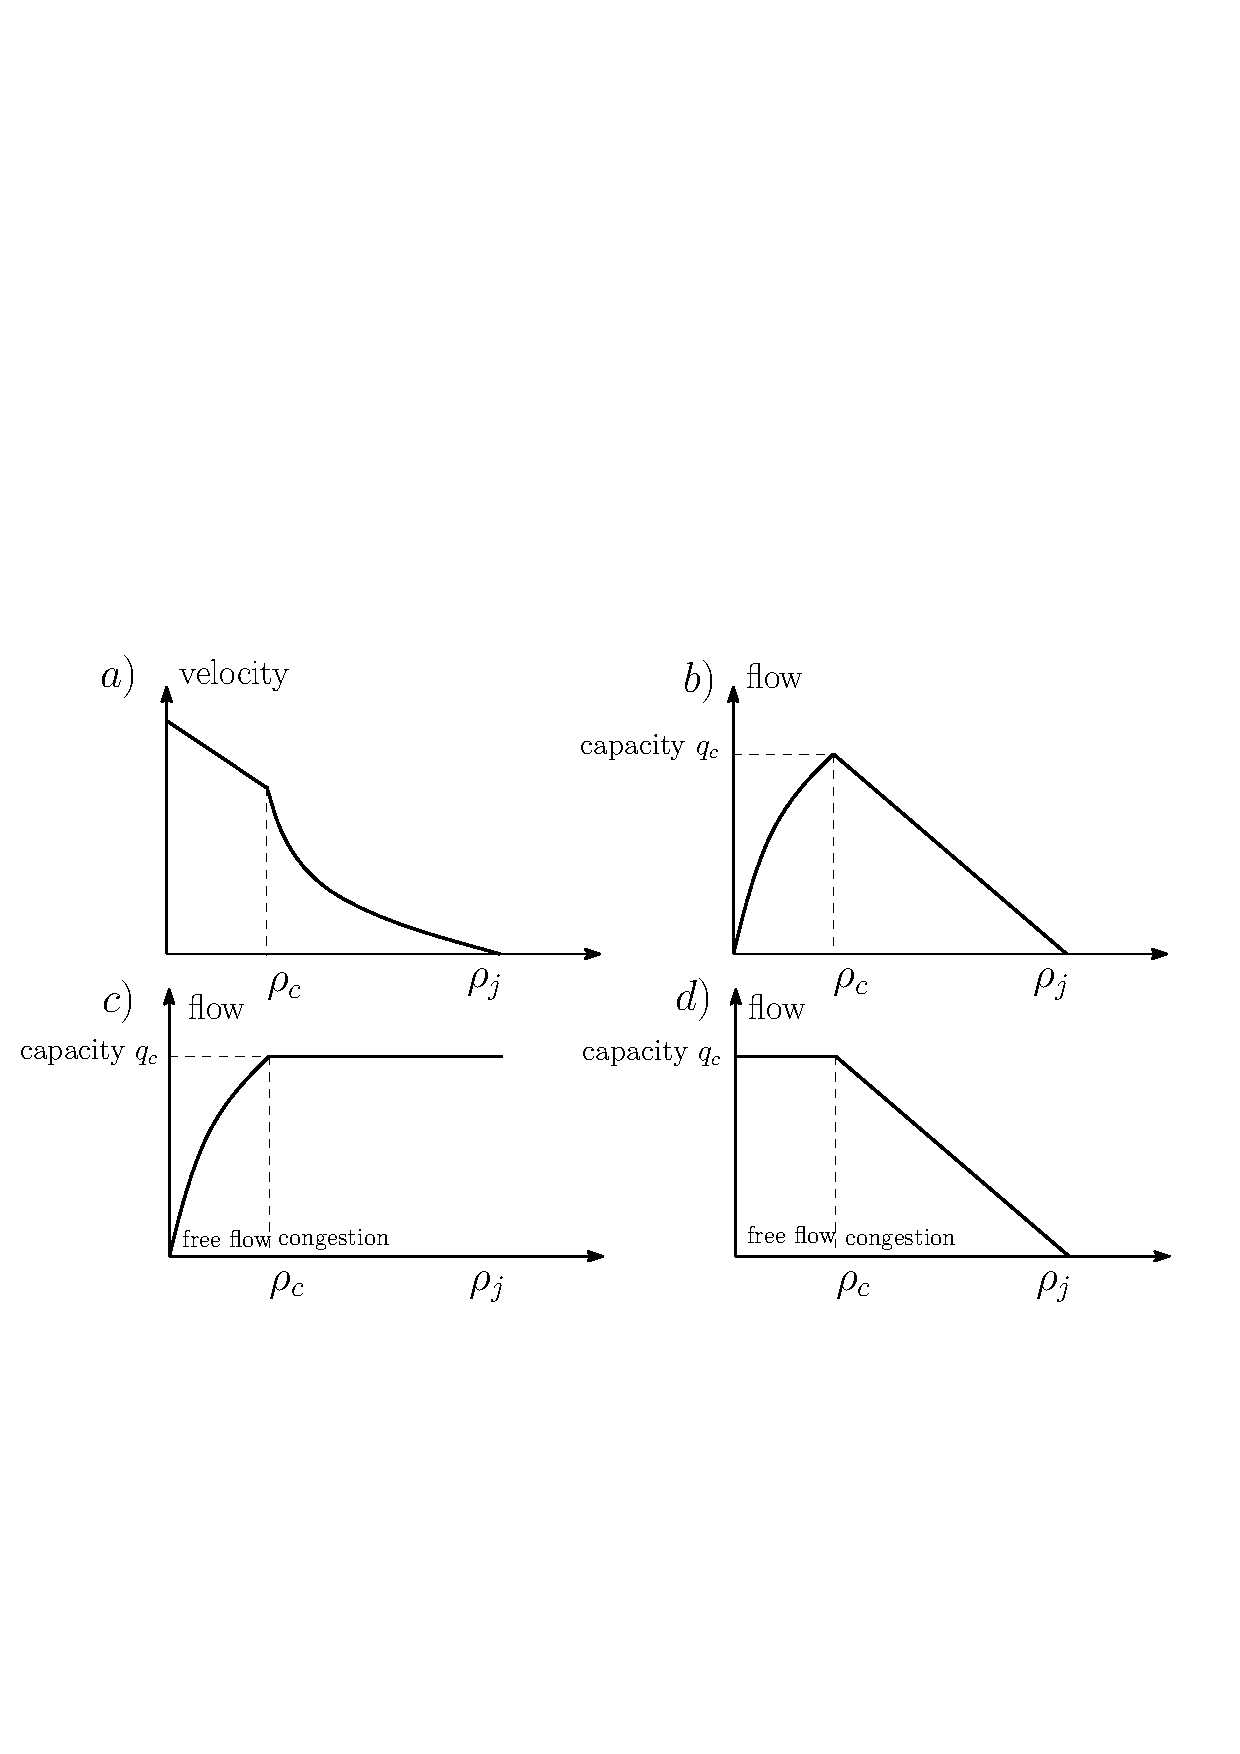
\includegraphics[width=12cm\textwidth]{fundamentalDiagramLH.pdf}
    \caption{a) Sending and receiving flows for the linear-hyperbolic velocity function.}
    \label{fig:fundamentalDiagramLH}
\end{figure}

In the context of the traffic model for velocity data assimilation \cite{Work2010}, the Daganzo-Newell velocity function is approximated by a linear-hyperbolic velocity function, with a linear expression in free-flow ($\rho \leq \rho_{c}$) and a hyperbolic expression in congestion ($\rho > \rho_{c}$) in order to have an invertible velocity function:

\begin{equation} \label{eq:lhVelocity}
v = V_{LH}(\rho) = \left\{ \begin{array}{rcl}
v_{f} \left( 1 - \frac{\rho}{\rho_{j}} \right) & if & \rho \leq \rho_{c} \\
-\omega_{f} \left( 1 - \frac{\rho_{j}}{\rho} \right) & if & \rho > \rho_{c}
\end{array}\right
\end{equation}

\noindent where $v_{c}$ is the critical velocity $v_{c} = V(\rho_{c})$. For continuity of the flux at the critical density $\rho_{c}$, the additional relation $\frac{\rho_{c}}{\rho_{j}} = \frac{\omega_{f}}{v_{f}}$ must be satisfied. The corresponding flux function is:

\begin{equation} \label{eq:lhFlux}
Q_{LH}(\rho) = \rho V_{LH}(\rho) = \left\{ \begin{array}{rcl}
v_{f} \left\rho( 1 - \frac{\rho}{\rho_{j}} \right) & \text{if} & \rho \leq \rho_{c} \\
-\omega_{f} \left( \rho - \rho_{j} \right) & \text{if} & \rho > \rho_{c}
\end{array}\right
\end{equation}

\noindent The sending and receiving flows for the linear-hyperbolic velocity function is:

\begin{equation} \label{eq:sendingFlow3}
S_{1}(\rho) = \left\{ \begin{array}{lll}
v_{f1} \left\rho( 1 - \frac{\rho}{\rho_{j1}} \right) & \text{if} & \rho \leq \rho_{c1} \\
q_{c1} &  \text{if} & \rho > \rho_{c1}
\end{array}\right
\end{equation}

\begin{equation} \label{eq:receivingFlow3}
R_{2}(\rho) = \left\{ \begin{array}{lll}
q_{c2} & \text{if} & \rho \leq \rho_{c2} \\
-\omega_{f2} \left( \rho - \rho_{j2} \right) &  \text{if} & \rho > \rho_{c2}
\end{array}\right
\end{equation}

\noindent When the velocity is a linear-hyperbolic velocity function (\ref{eq:lhVelocity}), and with the same assumptions (CTM framework and no capacity drop), the Godunov Flux becomes:

\begin{equation} \label{eq:rhoGodunovFlux3}
G_{DN}(\rho_{1},\rho_{2}) = \left\{ \begin{array}{lll}
-\omega_{f2} \left( \rho_{2} - \rho_{j2} \right) & \text{if} & (\rho_{1},\rho_{2}) \in \text{white region}\\
q_{c} & \text{if} & (\rho_{1},\rho_{2}) \in \text{light region}\\
v_{f1} \left\rho( 1 - \frac{\rho}{\rho_{j1}} \right) & \text{if} & (\rho_{1},\rho_{2}) \in \text{dark region}
\end{array}\right
\end{equation}

\noindent We can decompose in 7 modes:

\begin{table}[here]
\centering % used for centering table
\begin{tabular}{c c c c} % centered columns (4 columns)
\hline\hline %inserts double horizontal lines
Mode & $f_{LH}(\rho_{-},\rho,\rho_{+})$ \\ [0.5ex]% inserts table
%heading
\hline % inserts single horizontal line
1 & (1 - \alpha \omega_{f})\rho + \alpha \omega_{f} \rho_{+}\\ [1ex]
2 & (1 - \alpha \omega_{f})\rho + \alpha \omega_{f} \rho_{c}\\ [1ex]
3 & \rho + \alpha \omega_{f}\rho_{+} - \alpha \omega_{f}\rho_{c}\\ [1ex]
4 & (1 - \alpha v_{f})\rho + \alpha \frac{v_{f}}{\rho_{j}} \rho^{2} + \alpha v_{f} \rho_{c}\\ [1ex]
5 & \alpha v_{f} \rho_{-}(1-\frac{\rho_{-}}{\rho_{j}}) + \rho + \alpha \omega_{f} \rho_{+} - \alpha \omega_{f} \rho_{j}\\ [1ex]
6 & \alpha v_{f} \rho_{-}(1-\frac{\rho_{-}}{\rho_{j}}) + \rho - \alpha v_{f} \rho_{c}\\ [1ex]
7 & \alpha v_{f} \rho_{-}(1-\frac{\rho_{-}}{\rho_{j}}) + (1 - \alpha v_{f}) \rho + \alpha \frac{v_{f}}{\rho_{j}} \rho^{2}\\ [1ex]% [1ex] adds vertical space
\hline %inserts single line
\end{tabular}
\label{table:modesLH} % is used to refer this table in the text
\caption{Different values of $\rho^{t+1} = f(\rho_{-},\rho,\rho_{+})$ for the Linear-hyperbolic velocity function ($f_{LH}$).}
\end{table}

The sending flow is a parabolic function of the density as shown in Figure \ref{fig:fundamentalDiagramLH}, and so the Godunov scheme decomposed in different ''modes'' has some parabolic components as shown in Table \ref{table:modesLH}. However, the calibration of the fundamental diagram given flow measurements empirically shows that the \textit{sending flow} component is almost linear.

\begin{figure}[here]
  \centering
    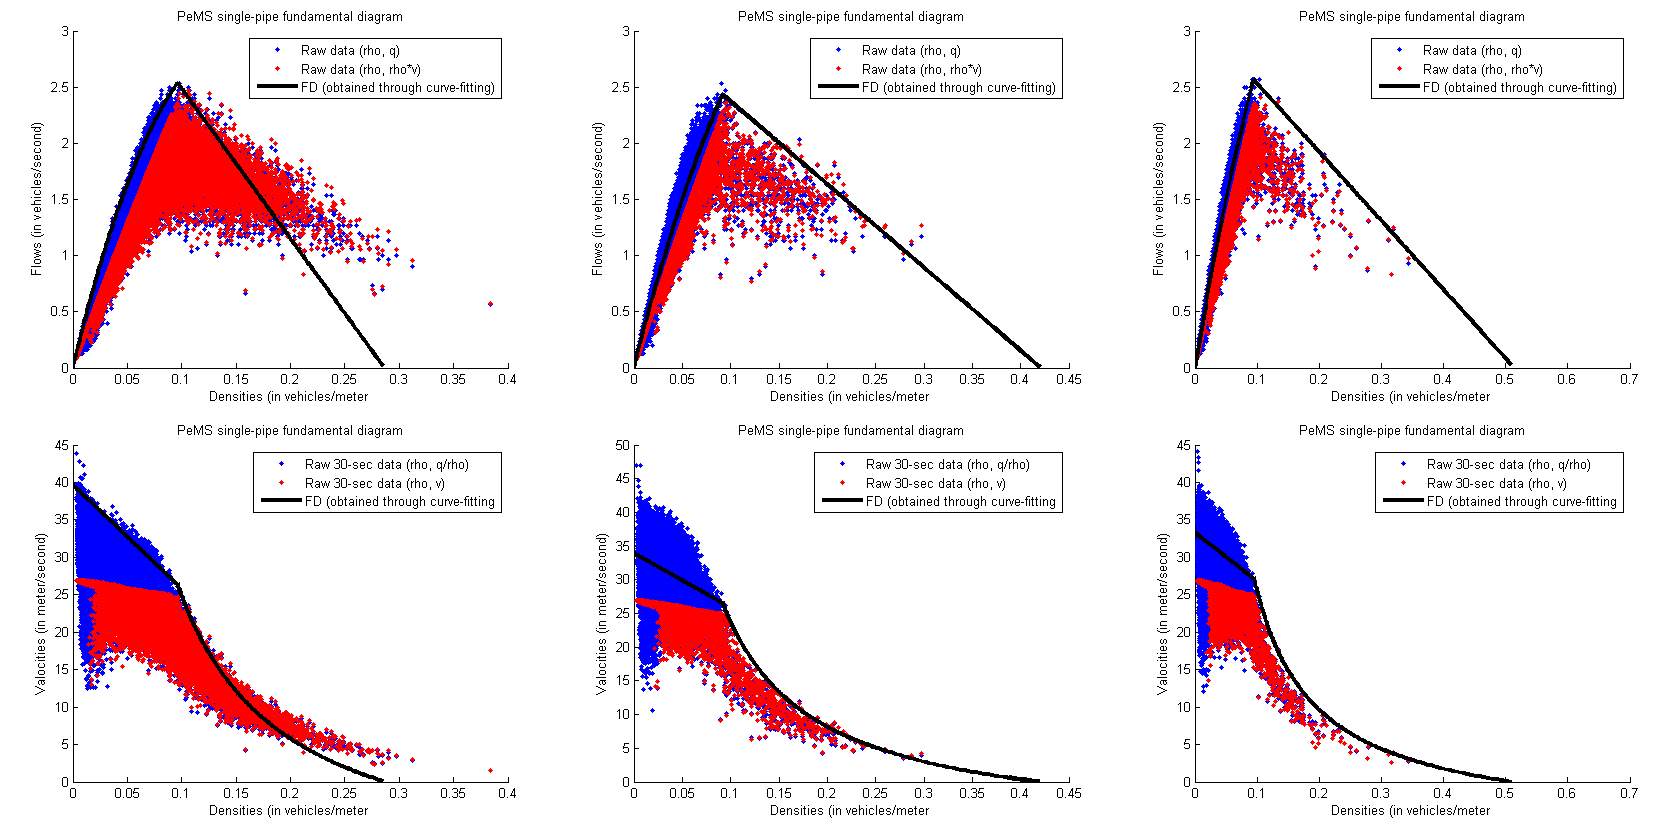
\includegraphics[width=15cm\textwidth]{calibration.png}
    \caption{Calibrated fundamental diagram.}
    \label{fig:calibration}
\end{figure}

\begin{table}[here]
\centering % used for centering table
\begin{tabular}{c c c c c c} % centered columns (4 columns)
\hline\hline %inserts double horizontal lines
PeMS id & 400041 & 400137 & 400141 & 400180 & 400189 \\ [0.5ex]% inserts table
%heading
\hline % inserts single horizontal line
v_{f} \quad (m/s) & 39.6631 & 33.9159 & 33.2646 & 30.0710 & 33.1679\\ [1ex]
\omega_{f} \quad (m/s) & 13.3431 & 7.3998 & 6.1202 & 6.4434 & 9.0381\\ [1ex]
\rho_{j} \quad (vehicles/m) & 0.2861 & 0.4206 & 0.5139 & 0.6321 & 0.3701\\ [1ex]
q_{c} \quad (vehicles/s) & 2.5333 & 2.4333 & 2.5667 & 3.2000 & 2.4333\\ [1ex]
\rho_{c} \quad (vehicles/m) & 0.0963 & 0.0918 & 0.0946 & 0.1354 & 0.1008\\ [1ex]
\rho_{c}/\rho_{j} & 0.3366 & 0.2183 & 0.1841 & 0.2142 & 0.2724\\ [1ex]
R^{2} & 0.983 & 0.995 & 0.997 & 0.995 & 0.991\\ [1ex]
\hline %inserts single line
\end{tabular}
\label{table:calibration} % is used to refer this table in the text
\caption{Calibrated parameters of the fundamental diagram (with a linear-hyperbolic velocity function) given PeMS measurements from five stations along the I-880 for the freeflow velocity $v_{f}$, the backwave velocity $\omega_{f}$, the jam density $\rho_{j}$, the flow capacity $q_{c}$, and the density capacity $\rho_{c}$.}
\end{table}

The California Freeway Performance Measurement System stores real-time data from 26,000 loop detectors \cite{Chen2005}. PeMS data is accessed via an internet browser (http://pems.eecs.berkeley.edu/). Such rich data set has been used to formulate and address practical questions in freeway modelling. In \cite{Dervisoglu2008}, a method for automated, empirical calibration of freeway traffic flow characteristics is presented. The method was used to calibrate a cell transmission model of Interstate-880 in San Francisco Bay Area, California, a 40-mile long urban freeway with lots of recurrent and non-recurrent congestion and with dozens of loop detector stations. For the purpose of our study, the method was modified to calibrate the traffic flow characteristics for a linear-hyperbolic velocity function (\ref{eq:lhVelocity}). The calibrated fundamental diagrams and velocity functions are presented in Figure \ref{fig:calibration}, and the calibrated parameters are presented in Table \ref{table:calibration}. 

From Equation \ref{eq:lhFlux}, the maximum contribution of the quadratic component over the linear one is given by $\rho_{c}/\rho_{j}$, which values have been obtained empirically from the calibrated parameters in Table \ref{table:calibration}. One way to test if the first order Taylor Series expansion of the prediction operator is a good linear approximation of $F_{LH}[.]$ is to fit a linear model to the parabole using the \textit{least squares linear regression}, and compute the \textit{coefficient of determination} $R^{2}$. As shown in Table \ref{table:calibration}, $R^{2}$ is very close to one, which means that the linear model is a good fit. Consequently, the first order multivariate Taylor Series expansion applied to each mode of the dynamic model is a good approximation, giving a PWA model.

\section{The case of capacity drop}\label{sec:CDFD}

In this section, we relax the constraint of no capacity drop made previously on the CTM. At a boundary between two cells, the upstream capacity $q_{c1}$ and the downstream capacity $q_{c2}$ can be different. We have a different Godunov flux. Figure \ref{fig:godunovDiagram} shows the explicit values taken by $G(\rho_{1},\rho_{2})$ in different regions of the space $(\rho_{1},\rho_{2})$ when $q_{c1} < q_{c2}$:

\begin{figure}[here]
  \centering
    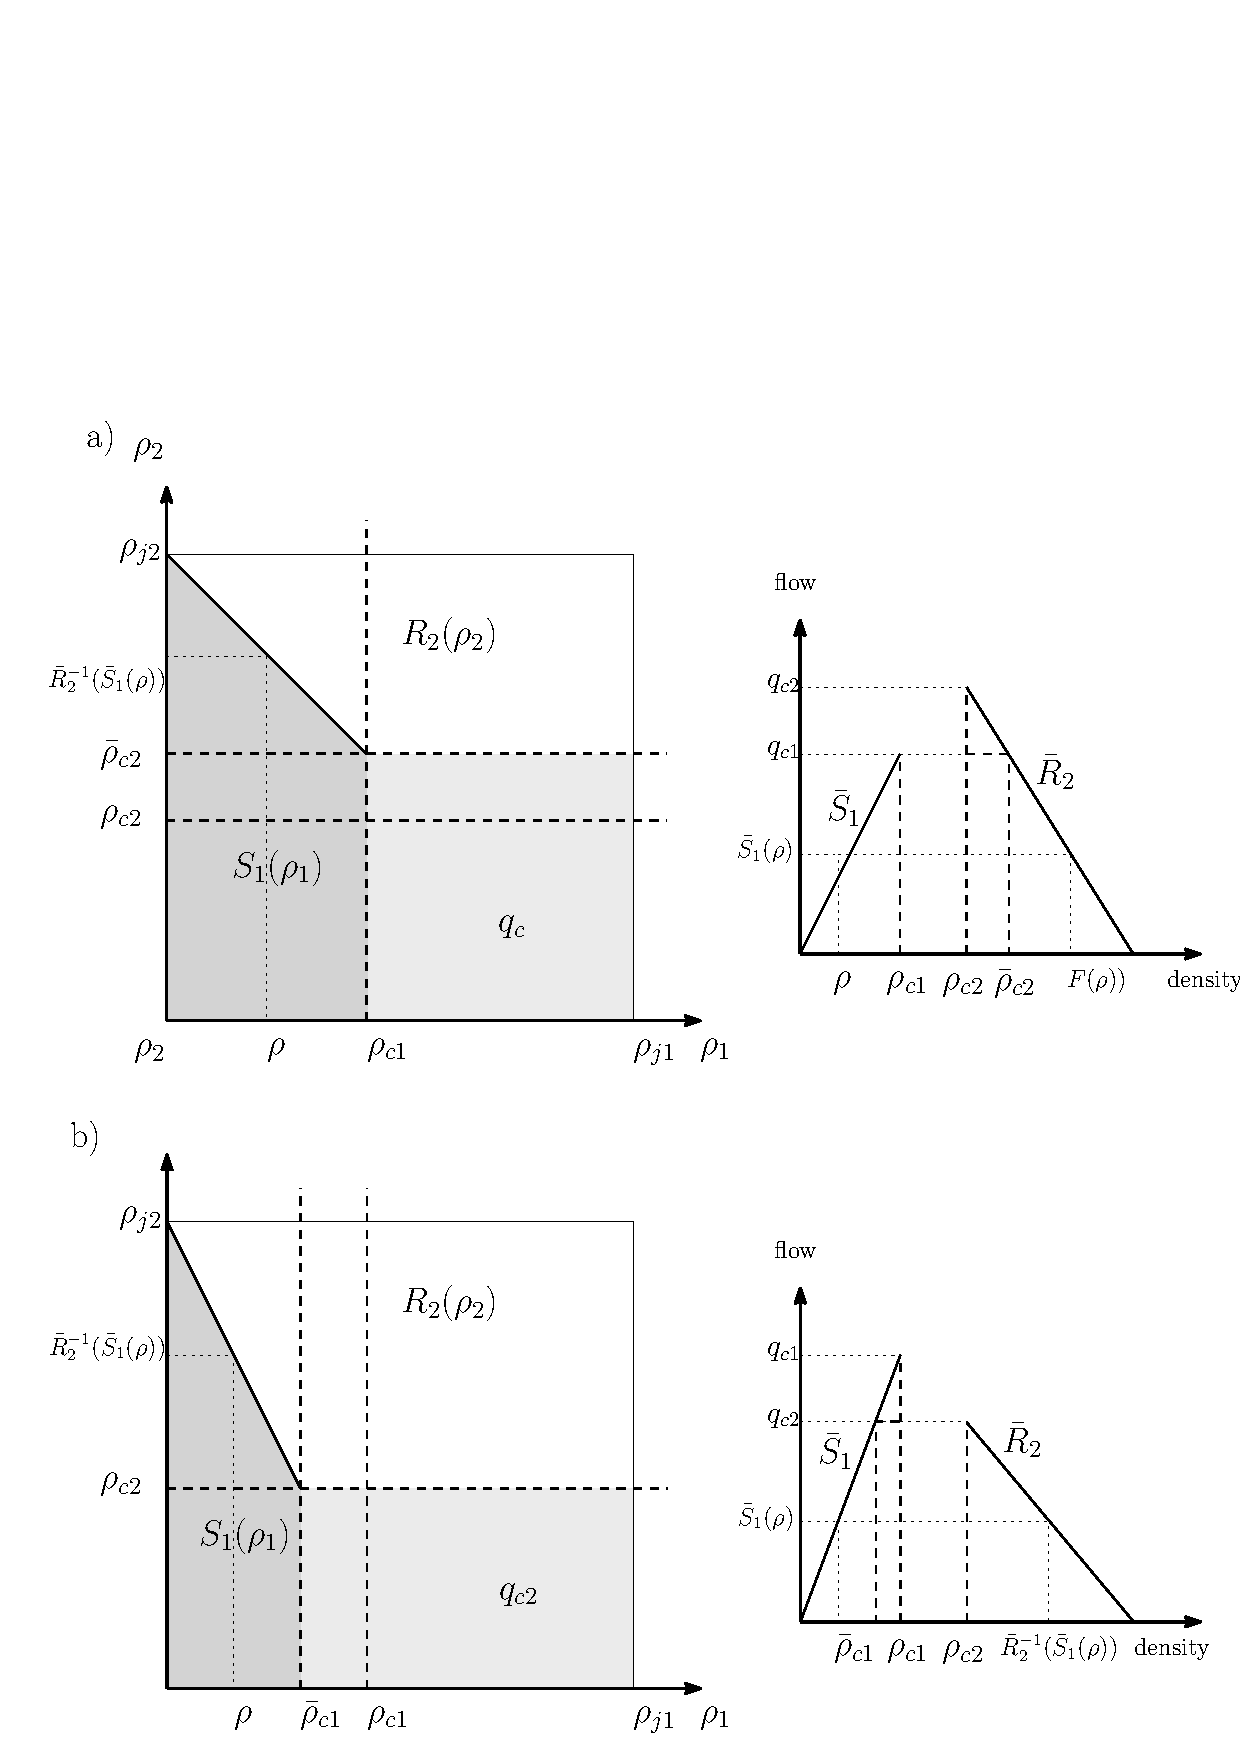
\includegraphics[width=15cm\textwidth]{godunovDiagram3.pdf}
    \caption{Values of $G(\rho_{1},\rho_{2})$ in the space $(\rho_{1},\rho_{2})$ for the Daganzo-Newell fundamental diagram with capacity drop $q_{c1} < q_{c2}$. Note that for illustration purposes we suppose $\rho_{c1}\leq\rho_{c2}$.}
    \label{fig:godunovDiagram}
\end{figure}

\noindent We note that the critical density $\rho_{c2}$ is increased to the \textit{effective} value $\bar{\rho}_{c2}$ for the receiving flow $R_{2}$, with $\bar{\rho}_{c2} = \bar{R}^{-1}_{2}(q_{c1})$, and the capacity is $q_{c1}$, which is the capacity of the sending flow $S_{1}$. And Figure \ref{fig:godunovDiagram} shows the explicit values taken by $G(\rho_{1},\rho_{2})$ in different regions of the space $(\rho_{1},\rho_{2})$ when $q_{c1} > q_{c2}$:

\begin{figure}[here]
  \centering
    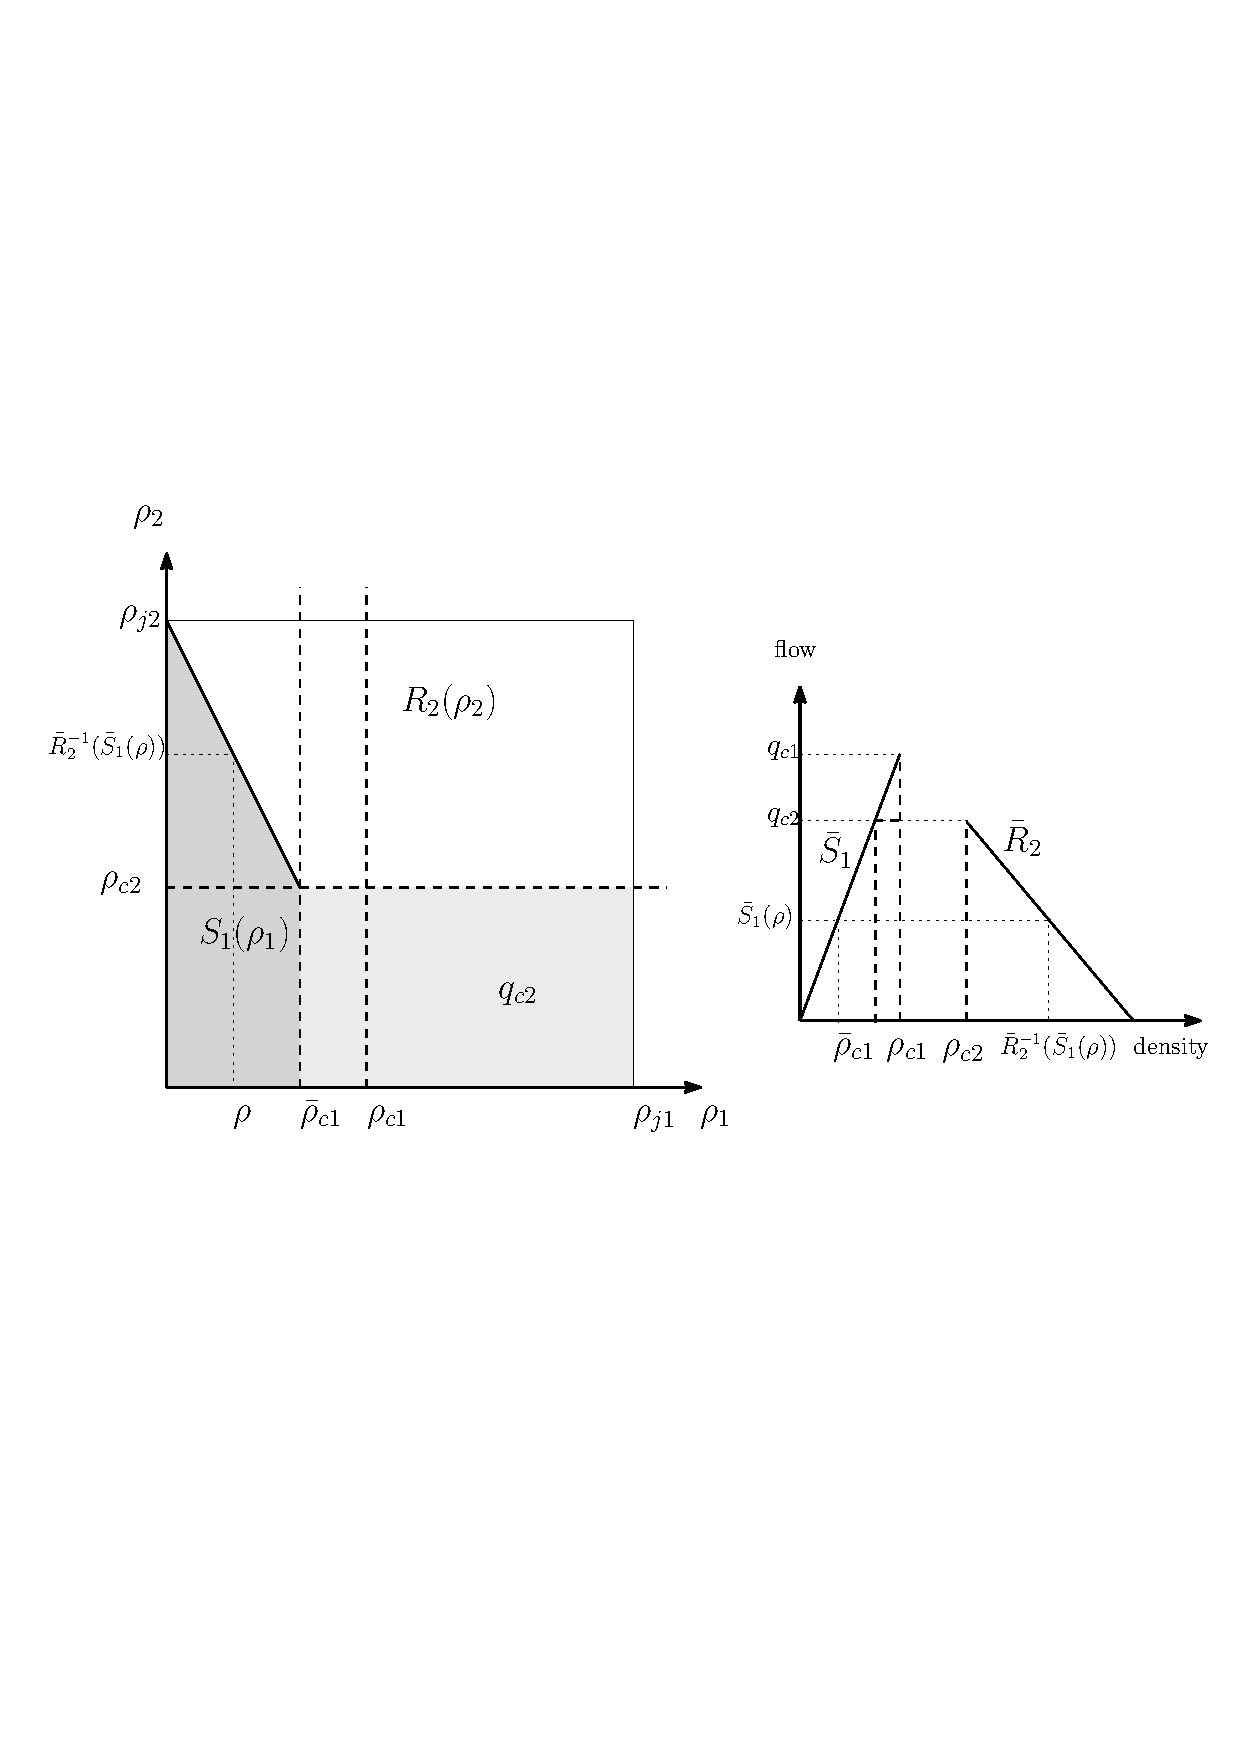
\includegraphics[width=15cm\textwidth]{godunovDiagram4.pdf}
    \caption{Values of $G(\rho_{1},\rho_{2})$ in the space $(\rho_{1},\rho_{2})$ for the Daganzo-Newell fundamental diagram with capacity drop $q_{c1} > q_{c2}$. Note that for illustration purposes we suppose $\rho_{c1}\leq\rho_{c2}$.}
    \label{fig:godunovDiagram}
\end{figure}

\noindent The critical density $\rho_{c1}$ is decreased to the \textit{effective} value $\bar{\rho}_{c1}$ for the sending flow $S_{1}$ with $\bar{\rho}_{c1} = \bar{S}^{-1}_{1}(q_{c2})$, and the capacity is $q_{c2}$, which is the capacity of the receiving flow $R_{2}$. At cell $i$, this implies the effective density $\bar{\rho}^{u}_{ci}$ associated with the upstream boundary can be different from the effective density $\bar{\rho}^{d}_{ci}$ associated with the downstream boundary, depending of the capacity drops at these boundaries. Hence, using the notations introduced in section \ref{sec:decompositionModes} all the combinations between $(\rho_{-},\rho)$ and $(\rho,\rho_{+})$ can be possible so we have nine modes. The table below describes the nine modes, where $q_{cu}$ is the capacity upstream for the Godunov flux $G(\rho_{-},\rho)$, and $q_{cd}$ is the capacity downstream for the Godunov flux $G(\rho,\rho_{+})$.

\begin{table}[here]
\centering % used for centering table
\begin{tabular}{c c c c c c} % centered columns (4 columns)
\hline\hline %inserts double horizontal lines
Mode & (\rho_{-}, \rho) & (\rho, \rho_{+}) & $f$(\rho_{-},\rho,\rho_{+}) & $f_{CD}$(\rho_{-},\rho,\rho_{+}) & State \\ [0.5ex]% inserts table
%heading
\hline % inserts single horizontal line
1 & W & W & \rho - \alpha(R_{+}(\rho_{+})-R(\rho)) & (1 - \alpha \omega_{f})\rho + \alpha \omega_{f} \rho_{+} & congestion\\ [1ex]
2 & W & L & \rho - \alpha(q_{cd}-R(\rho)) & (1 - \alpha \omega_{f})\rho + \alpha \omega_{f} \rho_{c} & congestion\\ [1ex]
3 & L & W & \rho - \alpha(R_{+}(\rho_{+})-q_{cu}) & \rho + \alpha \omega_{f}\rho_{+} - \alpha \omega_{f}\rho_{c} & congestion\\ [1ex]
4 & L & D & \rho - \alpha(S(\rho)-q_{cu}) & (1 - \alpha v_{f})\rho + \alpha v_{f} \rho_{c} & free flow\\ [1ex]
5 & D & W & \rho - \alpha(R_{+}(\rho_{+})-S_{-}(\rho_{-})) & \alpha v_{f} \rho_{-} + \rho + \alpha \omega_{f} \rho_{+} - \alpha \omega_{f} \rho_{j} & critical\\ [1ex]
6 & D & L & \rho - \alpha(q_{cd}-S_{-}(\rho_{-})) & \alpha v_{f} \rho_{-} + \rho - \alpha v_{f} \rho_{c} & free flow\\ [1ex]
7 & D & D & \rho - \alpha(S(\rho)-S_{-}(\rho_{-})) & \alpha v_{f} \rho_{-} + (1 - \alpha v_{f})\rho & free flow\\ [1ex]
8 & W & D & \rho - \alpha(S{\rho}-R(\rho)) & (1 - \alpha v_{f} - \alpha \omega_{f})\rho  + \alpha \omega_{f}\rho_{j} & critical\\[1ex]
9 & L & L & \rho - \alpha(q_{cu}-q_{cd}) & \rho - \alpha(q_{cu}-q_{cd}) & critical\\[1ex]
\hline %inserts single line
\end{tabular}
\label{table:nineModes} % is used to refer this table in the text
\caption{Different values of $\rho^{t+1} = f(\rho_{-},\rho,\rho_{+})$ depending on the values of $G(\rho_{-},\rho)$ and $G(\rho,\rho_{+})$ in the space $(\rho_{1},\rho_{2})$ in the case of capacity drop.}
\end{table}

\bibliography{myBiblio}
\bibliographystyle{plain}

\end{document}
